\section{Experimental Study}
\label{sec-exp}

We evaluate \sys along five research questions.
\begin{itemize}
\item \textbf{[RQ1] The store}: how does a B+ tree store with three
  permutations compare with an LSM-based, a Java B+ tree, and a relational
  store on triple patterns, queries, and loading?
\item \textbf{[RQ2] Hierarchies}: what do interval labels cost, and how do they
  compare with materializing and rewriting, and with other engines'
  subclass-path queries?
\item \textbf{[RQ3] Vector indexes}: what recall, time, and memory do the
  four indexes give on real embeddings?
\item \textbf{[RQ4] Filtered search}: which strategy answers
  $\mathrm{near}(q,c,k)$ fastest, and does a single rule choose well?
\item \textbf{[RQ5] Concurrency}: how do lookups and inserts scale with the
  number of threads, and what do readers see while a writer runs?
\item \textbf{[RQ6] Design choices}: what do three permutations, the bulk
  loader, and the decode cache each buy?
\end{itemize}

Table~\ref{tab-glance} summarizes the answers; the subsections give every
measurement.

\begin{table}[t]
\caption{Selected results: how many times faster \sys{} is than each other engine (the time of the other engine divided by \sys's; for throughput, \sys's divided by the other's). All tables of this section give every measurement.}
\label{tab-glance}
\small
\resizebox{\columnwidth}{!}{%
\begin{tabular}{@{}lrrrr@{}}
\toprule
 & Ox.\ RocksDB & Ox.\ memory & Jena TDB2 & SQLite \\
\midrule
pattern $(s,\cdot,\cdot)$ & 8.4$\times$ & 3.4$\times$ & 36.7$\times$ & 4.2$\times$ \\
pattern $(s,p,\cdot)$ & 7.2$\times$ & 4.6$\times$ & 27.3$\times$ & 5.5$\times$ \\
LUBM query 1 & 3.7$\times$ & 1.4$\times$ & 58.4$\times$ & 2.0$\times$ \\
instances of a class, 10--99 below & 39.1$\times$ & 7.7$\times$ & 47.9$\times$ & 14.9$\times$ \\
instances of a class, 1000+ below & 5.8$\times$ & 2.2$\times$ & 5.3$\times$ & 3.5$\times$ \\
lookups per second, 8 threads & 7.0$\times$ & 3.2$\times$ & 6.1$\times$ & 3.9$\times$ \\
lookups per second, 8 readers + 1 writer & 10.2$\times$ & 4.8$\times$ & 18.8$\times$ & 4.3$\times$ \\
\bottomrule
\end{tabular}}
\end{table}


\subsection{Experimental Setup}

\stitle{Systems}.
We compare \sys, built in release mode with the B+ tree store (SPO, POS, OSP),
a 256\,MiB buffer pool, and automatic join selection, with four configurations
of three other systems, all run in-process on one thread of the same
machine: Oxigraph 0.5.13~\cite{oxigraph} through its Rust interface, with
RocksDB on disk and with its in-memory store; Apache Jena TDB2
5.2.0~\cite{jenatdb} on Java 17 with a 4\,GiB heap and its own bulk loader;
and SQLite 3.51 with one table of three string columns, a primary key on
$(s,p,o)$ and two more indexes on $(p,o,s)$ and $(o,s,p)$, a SPARQL basic
graph pattern translated into a join of the table with itself, and
\texttt{ANALYZE} after loading.
SQLite stores terms as strings and \sys as ids; we include it as the
relational baseline.
RDF4J, QLever, and RDFox are discussed in Section~\ref{sec-related} but not run.
Concurrency is measured in-process: threads for \sys, Oxigraph, and Jena, and
processes with one connection each for SQLite, whose Python driver would
otherwise share one interpreter lock.

\stitle{Data}.
LUBM~\cite{lubm} at one and ten universities (103,104 and 1,316,700
statements) and the Gene Ontology~\cite{ashburner2000} (release 2026-07-26
without obsolete terms: 38,092 classes, 57,456 \texttt{is\_a} edges) with
$d=384$ embeddings of the term names by
\texttt{all-MiniLM-L6-v2}~\cite{reimers2019}.
Because the Gene Ontology has no instances, we add 200,000 synthetic
entities of one to three types drawn uniformly from its classes (495,552
triples in all).

\stitle{Workloads and method}.
The pattern workload samples, from each dataset, 100 constants for every
bound position of each shape of Table~\ref{tab-perms}, so that every shape is
measured; the LUBM workload is the 14 queries of the benchmark.
The instance workload asks for $\mathrm{inst}(c)$ for 30 classes in each of
five size buckets, answered by \sys through interval scans and by the others
through the subclass path \texttt{?c rdfs:subClassOf* c . ?x a ?c} (SQLite: a
recursive query).
Each query is parsed once, run to warm the caches (three times for the JVM and SQLite), and then five to nine times; we report the median, and the mean of
medians over a workload.
Every engine converts each answer to its string, and the row counts of all
engines agree on every query.
Queries that run for a minute are reported as timeouts; none did.
Times are warm: they include \sys's decode cache and the other engines' own
caches.
The machine is an Apple M2 Pro with 16\,GiB.
Counts of page reads use a cold 64-frame pool.
The code, data generators, and every number in this section are available
at the artifact URL.

\subsection{RQ1: The Store}

Table~\ref{tab-load} gives the cost of loading LUBM(10), and
Table~\ref{tab-queries} the query times.

\begin{table}[t]
\caption{Loading LUBM in each engine (bulk loader, one thread of the loader, files on a local SSD). Oxigraph's count is distinct triples; \sys's is statements read.}
\label{tab:load}
\small
\resizebox{\columnwidth}{!}{%
\begin{tabular}{@{}llrrrr@{}}
\toprule
Data & Engine & triples & load (s) & disk (MiB) & RSS (MiB) \\
\midrule
LUBM(1) & \sys{} & 103\,104 & 1.02 & 10.8 & 322 \\
 & Oxigraph, RocksDB & 100\,573 & 0.13 & 17.8 & 60 \\
 & Oxigraph, memory & 100\,573 & 0.18 & --- & 53 \\
\midrule
LUBM(10) & \sys{} & 1\,316\,700 & 13.83 & 133.7 & 637 \\
 & Oxigraph, RocksDB & 1\,272\,953 & 1.95 & 176.3 & 87 \\
 & Oxigraph, memory & 1\,272\,953 & 2.32 & --- & 546 \\
\bottomrule
\end{tabular}}
\end{table}


\begin{table*}[t]
\caption{Query times on LUBM(10): the mean over 100 sampled constants per pattern shape (all 18 predicates for $(\cdot,p,\cdot)$), and the median of the four LUBM queries that return rows without inference. Row counts agree across engines.}
\label{tab-queries}
\small
\begin{tabular}{@{}lrrrrrr@{}}
\toprule
Query & rows & \sys{} & Ox.\ RocksDB & Ox.\ memory & Jena TDB2 & SQLite \\
\midrule
$(s,\cdot,\cdot)$ & 7 & 3\,$\mu$s & 27\,$\mu$s & 11\,$\mu$s & 117\,$\mu$s & 13\,$\mu$s \\
$(s,p,\cdot)$ & 2 & 2\,$\mu$s & 14\,$\mu$s & 9\,$\mu$s & 52\,$\mu$s & 11\,$\mu$s \\
$(\cdot,\cdot,o)$ & 16,233 & 11.0\,ms & 35.7\,ms & 10.4\,ms & 23.7\,ms & 8.4\,ms \\
$(\cdot,p,o)$ & 16,225 & 10.2\,ms & 19.4\,ms & 7.8\,ms & 24.8\,ms & 6.2\,ms \\
$(\cdot,p,\cdot)$ & 70,720 & 70.8\,ms & 161.2\,ms & 41.2\,ms & 107.5\,ms & 35.5\,ms \\
\midrule
LUBM 1 & 4 & 9\,$\mu$s & 32\,$\mu$s & 12\,$\mu$s & 508\,$\mu$s & 18\,$\mu$s \\
LUBM 3 & 6 & 11\,$\mu$s & 37\,$\mu$s & 13\,$\mu$s & 234\,$\mu$s & 18\,$\mu$s \\
LUBM 2 (triangle) & 28 & 8.2\,ms & 275.1\,ms & 34.1\,ms & 120.1\,ms & 4.0\,ms \\
LUBM 14 (scan) & 75,547 & 46.0\,ms & 88.1\,ms & 40.8\,ms & 138.7\,ms & 29.3\,ms \\
\bottomrule
\end{tabular}
\end{table*}


\stitle{Selective patterns}.
For patterns that bind the subject, \sys takes 3\,$\mu$s and 2\,$\mu$s and the
others 11 to 117\,$\mu$s and 9 to 52\,$\mu$s: \sys is 3.4 to 37$\times$ faster
on $(s,\cdot,\cdot)$ and 4.6 to 27$\times$ on $(s,p,\cdot)$, and 1.4 to
58$\times$ faster on the selective LUBM queries.
Every answer is one descent of a B+ tree that fits the pool and a few keys.

\stitle{Large results}.
For patterns that return 16,000 to 71,000 rows, \sys takes 10 to 71\,ms: 1.9 to
3.2$\times$ faster than Oxigraph on RocksDB, 1.5 to 2.4$\times$ faster than
Jena, equal to Oxigraph's in-memory store on $(\cdot,\cdot,o)$ and 1.3 to
1.7$\times$ slower on the other two, and 1.3 to 2.0$\times$ slower than SQLite,
whose string index returns spellings without a dictionary.

\stitle{LUBM queries}.
Ten of the fourteen LUBM queries return no rows without inference; every
engine answers them in microseconds and the ratios of two tiny times mean
nothing, so Table~\ref{tab-queries} lists the four that return rows.
On the triangle query SQLite takes 4.0\,ms, \sys 8.2\,ms, Oxigraph in memory
34\,ms, Jena 120\,ms, and Oxigraph on RocksDB 275\,ms: \sys is 33$\times$
faster than the last, and twice as slow as SQLite; we did not inspect the
other engines' plans.
On the large scan (LUBM 14) the order is SQLite, Oxigraph in memory, \sys,
Oxigraph on RocksDB, Jena.

\stitle{Loading}.
\sys is the slowest to load, 11.4\,s against 2.0\,s for Oxigraph on RocksDB
(5.6$\times$), 6.1\,s for Jena, and 8.1\,s for SQLite, and its peak
memory is 584\,MiB against 78\,MiB for Oxigraph on RocksDB, because it
parses RDF/XML through a C library, interns each term through two B+ trees,
and builds exact statistics.
Its file is the smallest, 134\,MiB against 176 for Oxigraph on RocksDB, 363
for Jena, and 706 for SQLite.
In sum, a B+ tree store of three permutations is competitive with the
other designs on basic graph patterns: fastest on selective ones, within a
factor of two of the best on large ones, and slowest to load.

\subsection{RQ2: Hierarchies}

\stitle{Interval labels}.
Table~\ref{tab-labels} shows that the Gene Ontology needs 76,570 intervals for
38,092 classes, 2.01 per class and 598\,KiB in all, where the closure it
replaces has 393,448 ancestor pairs (9\,MiB as 24-byte keys in one
permutation).
The choice of spanning forest matters little: taking the deepest parent saves
13\%.
The tail is long, one class needing 741 intervals, within the bound of
Lemma~\ref{lem-size}.
Labels build in 15\,ms, and asking whether a class is below another takes
27\,ns against 775\,ns for a search up the parents.

\begin{table}[t]
\caption{Interval labels for the Gene Ontology.}
\label{tab-labels}
\small
\resizebox{\columnwidth}{!}{%
\begin{tabular}{@{}lrrrr@{}}
\toprule
Spanning-forest rule & non-tree edges & intervals & mean / p99 / max & build \\
\midrule
deepest parent & 19,367 & 76,570 & 2.01 / 17 / 741 & 14.9 ms \\
first parent & 19,367 & 87,769 & 2.30 / 22 / 740 & 14.4 ms \\
\bottomrule
\end{tabular}}
\end{table}

\stitle{Against materializing and rewriting}.
Table~\ref{tab-desc} compares interval scans with a search that scans POS once
per class.
For a class with a thousand or more descendants the intervals need 101
scans instead of 3,304, 40 page reads instead of 694, and 0.5\,ms instead of
9\,ms.
Table~\ref{tab-types} compares the three strategies for instance queries on
the synthetic instances.
Materializing the closure turns 495,552 triples into 4,017,973 (8.1$\times$),
the file from 63.6 to 309.5\,MiB, and the load from 5.1 to 180\,s.
The interval index adds 9.3\,MiB (15\%) and 0.17\,s.
On queries the interval index is close to the materialized store and far from
rewriting: for a class with a thousand or more descendants it reads 265 pages
against 182 (materialized) and 12,803 (rewrite).
All three return identical answers on every sampled class.
On LUBM(1) the hierarchy is shallow (43 classes) and the three are within a
factor of about two on every query, and materialization adds 15\% to the
triples: the benefit of intervals grows with the depth and breadth of the
hierarchy.

\begin{table}[t]
\caption{Descendants of a class in GO, cold 64-frame pool, mean over up to 40 classes per row.}
\label{tab-desc}
\small
\begin{tabular}{@{}lrrrr@{}}
\toprule
Below $c$ & method & scans & page reads & $\mu$s \\
\midrule
10--99 & intervals & 5.9 & 5.8 & 59 \\
 & one scan per class & 30.6 & 16.3 & 149 \\
100--999 & intervals & 29.1 & 13.2 & 147 \\
 & one scan per class & 268.2 & 65.7 & 803 \\
1000+ & intervals & 101.3 & 40.1 & 528 \\
 & one scan per class & 3303.6 & 694.1 & 8998 \\
\bottomrule
\end{tabular}
\end{table}

\begin{table}[t]
\caption{Instances of $c$ on 200,000 synthetic entities over GO, mean over 30 classes per row (cold 64-frame pool). Top: cost of the store.}
\label{tab-types}
\small
\begin{tabular}{@{}lrrr@{}}
\toprule
Strategy & triples & file (MiB) & load (s) \\
\midrule
rewrite & 495,552 & 63.6 & 5.09 \\
intervals & 495,552 & 72.9 & 5.26 \\
materialize & 4,017,973 & 309.5 & 180.31 \\
\bottomrule
\end{tabular}

\medskip
\begin{tabular}{@{}lrrrr@{}}
\toprule
Below $c$ & strategy & answers & page reads & $\mu$s \\
\midrule
10--99 & intervals & 278 & 8.4 & 90 \\
 & rewrite & 278 & 87.5 & 571 \\
 & materialized & 278 & 6.6 & 444 \\
100--999 & intervals & 2,954 & 40.9 & 1,461 \\
 & rewrite & 2,954 & 1,153 & 7,280 \\
 & materialized & 2,954 & 22.5 & 987 \\
1000+ & intervals & 29,904 & 264.8 & 4,555 \\
 & rewrite & 29,904 & 12,803 & 82,441 \\
 & materialized & 29,904 & 182.0 & 3,776 \\
\bottomrule
\end{tabular}
\end{table}

\stitle{Against other engines}.
Table~\ref{tab-hier} compares \sys with the other engines on instance
queries.
The interval scan alone returns term ids, in 1.9\,ms for the 29,904 answers of
the largest classes (about 60\,ns each); returning strings, as the others do, takes
11.5\,ms because each id is decoded.
At the string level \sys is 2.2$\times$ faster than the best other engine
(Oxigraph in memory) on the largest classes, 3.5$\times$ faster than SQLite's
recursive query, and 5.4 to 5.8$\times$ faster than Jena and Oxigraph on
RocksDB, and 5 to 9$\times$ faster than Oxigraph in memory on classes with
fewer than 1,000 instances.
With the decode cache off (Table~\ref{tab-cache}) \sys takes 22.6\,ms for the
largest classes, still 1.1$\times$ faster than the best other engine.
A subclass path is evaluated by the others as a graph traversal followed by a
join, and by \sys as range scans of one tree that return disjoint answers.

\begin{table}[t]
\caption{Instances of a class and its subclasses, 200\,000 entities over the Gene Ontology, 30 classes per row, warm: mean time. \sys{} answers by interval scans; Oxigraph by \texttt{?x a ?c . ?c rdfs:subClassOf* <C>}. \sys{} ``ids'' stops before the dictionary; ``strings'' decodes every answer, as Oxigraph does.}
\label{tab:hier}
\small
\resizebox{\columnwidth}{!}{%
\begin{tabular}{@{}lrrrrr@{}}
\toprule
Below $C$ & answers & \sys{} ids & \sys{} strings & Ox., RocksDB & Ox., memory \\
\midrule
1 & 10 & 1\,$\mu$s & 11\,$\mu$s & 37\,$\mu$s & 13\,$\mu$s \\
2-9 & 40 & 3\,$\mu$s & 42\,$\mu$s & 91\,$\mu$s & 23\,$\mu$s \\
10-99 & 278 & 10\,$\mu$s & 275\,$\mu$s & 539\,$\mu$s & 110\,$\mu$s \\
100-999 & 2,954 & 127\,$\mu$s & 2.9\,ms & 5.4\,ms & 1.1\,ms \\
1000+ & 29,904 & 1.7\,ms & 29.1\,ms & 60.6\,ms & 21.8\,ms \\
\bottomrule
\end{tabular}}
\end{table}


\subsection{RQ3: Vector Indexes}

We ran 1,000 query terms (the term itself excluded from its answer) against
all 38,092 vectors, with exact search as ground truth.
Table~\ref{tab-knn} gives selected points and Figure~\ref{fig-knn} the
recall--latency curves.

\begin{table}[t]
\caption{Vector indexes on GO (recall@10, mean time per query, memory of the structure, build time).}
\label{tab-knn}
\small
\resizebox{\columnwidth}{!}{%
\begin{tabular}{@{}llrrrr@{}}
\toprule
Index & setting & recall & $\mu$s & MiB & build (s) \\
\midrule
flat float32 & exact & 1.000 & 2,238 & 55.8 & --- \\
flat 8-bit & exact over codes & 0.996 & 4,554 & 14.1 & --- \\
flat PQ $m{=}48$ & codes only & 0.778 & 819 & 1.7 & 10.4 \\
flat PQ $m{=}48$ & re-rank 100 & 0.998 & 905 & 1.7$^\dagger$ & 10.4 \\
IVF $\nu{=}512$ & $\rho{=}8$ & 0.892 & 149 & 56.5 & 17.5 \\
IVF $\nu{=}512$ & $\rho{=}16$ & 0.929 & 255 & 56.5 & 17.5 \\
IVF $\nu{=}512$ & $\rho{=}64$ & 0.976 & 928 & 56.5 & 17.5 \\
IVF $\nu{=}512$, 8-bit & $\rho{=}16$ & 0.926 & 263 & 14.8 & 17.5 \\
IVF $\nu{=}512$, PQ 96 & $\rho{=}16$ & 0.839 & 178 & 4.2 & 38.4 \\
HNSW $M{=}16$ & $\ef{=}10$ & 0.993 & 44 & 59.7 & 15.0 \\
HNSW $M{=}16$ & $\ef{=}40$ & 0.997 & 108 & 59.7 & 15.0 \\
HNSW $M{=}32$ & $\ef{=}160$ & 0.999 & 474 & 63.4 & 28.0 \\
\bottomrule
\end{tabular}}

\smallskip
{\footnotesize $^\dagger$ re-ranking reads the float vectors as well.}
\end{table}

\begin{figure}[t]
\centering
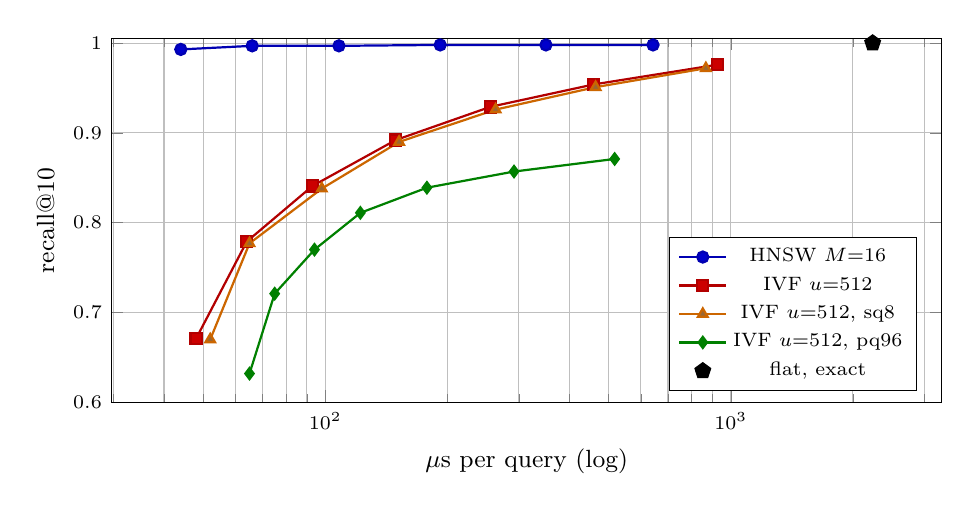
\begin{tikzpicture}
\begin{axis}[width=\columnwidth,height=6.2cm,xmode=log,xlabel={$\mu$s per query (log)},ylabel={recall@10},ymin=0.6,ymax=1.005,grid=both,legend pos=south east,legend style={font=\scriptsize},tick label style={font=\scriptsize},label style={font=\small}]
\addplot+[mark=*,color=blue!70!black,thick] coordinates {(44,0.993) (66,0.997) (108,0.997) (192,0.998) (350,0.998) (643,0.998)};
\addlegendentry{HNSW $M{=}16$}
\addplot+[mark=square*,color=red!70!black,thick] coordinates {(48,0.671) (64,0.779) (93,0.841) (149,0.892) (255,0.929) (459,0.954) (928,0.976)};
\addlegendentry{IVF $
u{=}512$}
\addplot+[mark=triangle*,color=orange!80!black,thick] coordinates {(52,0.67) (65,0.777) (98,0.838) (152,0.89) (263,0.926) (464,0.951) (868,0.972)};
\addlegendentry{IVF $
u{=}512$, sq8}
\addplot+[mark=diamond*,color=green!50!black,thick] coordinates {(65,0.632) (75,0.721) (94,0.77) (122,0.811) (178,0.839) (292,0.857) (517,0.871)};
\addlegendentry{IVF $
u{=}512$, pq96}
\addplot[only marks,mark=pentagon*,mark size=3pt,color=black] coordinates {(2238,1)};
\addlegendentry{flat, exact}
\end{axis}
\end{tikzpicture}

\caption{Recall@10 against time per query on GO (38,092 vectors, 384 dimensions).}
\label{fig-knn}
\end{figure}

\stitle{A baseline that is not slow by accident}.
Our first run scored with a plain dot-product loop.
A compiler may not vectorize it without \texttt{-ffast-math}, and the exact
scan took 8.3\,ms, which would have made the speed-ups look about twice as
large: HNSW at $\ef{=}10$ is 103 times faster than that baseline and 51 times
faster than the vectorized one.
With eight independent accumulators the exact scan takes 2.2\,ms (13
Gflop/s), and every number here uses that.
A speed-up over ``exact'' depends entirely on how fast exact is.

\stitle{What the numbers say}.
HNSW dominates on this data: recall 0.993 at 44\,$\mu$s, 51$\times$ faster
than the exact scan, for 3.9\,MiB of links on top of the vectors.
IVF needs 255\,$\mu$s for 0.929 and 928\,$\mu$s for 0.976.
IVF over the B+ tree is about 2.7$\times$ more expensive per scored row than a
contiguous scan (157\,ns against 59\,ns): each entry is a decoded 24-byte key
and a random read of the vector.
That is the price of lists that page, cache, and update with the triples.
The cost model holds in shape: more lists make a query cheaper until the
centroid scan dominates ($\nu{=}2048$ pays 124\,$\mu$s at $\rho{=}1$).
Product quantization is for memory, not speed, at this size: codes alone
reach 0.78 or 0.88 recall in 1.7 or 3.5\,MiB, and re-ranking the best 100
exactly recovers 0.998 and 1.000 but needs the float vectors.
8-bit codes keep 0.996 recall in a quarter of the memory and are slower than
float32, because converting bytes to floats costs more than the cache misses
they avoid at 56\,MiB.
The queries are terms of the ontology, whose neighbors are also terms of it;
queries from outside the vocabulary, such as free text, would be harder, and
we do not measure them.

\subsection{RQ4: Filtered Search}

For 20 classes in each of five size buckets we ran the ten nearest terms
under $c$ for a query inside $c$ and one outside it, against the exact answer
over the members.
IVF uses 512 lists and 16 probes, HNSW $M{=}16$ and $\ef{=}64$.
Table~\ref{tab-hybrid} gives recall and time.

\begin{table*}[t]
\caption{Ten nearest terms under a class $c$, by subtree size, query inside or outside $c$: recall@10 / $\mu$s per query. GO, 38,092 terms. Masked and post-filtered searches use the index; pre-filter resolves the members and scores them exactly.}
\label{tab-hybrid}
\small
\begin{tabular}{@{}lccccc@{}}
\toprule
Strategy & $\le$10 & 11--100 & 101--1000 & 1001--5000 & $>$5000 \\
\midrule
\multicolumn{6}{@{}l}{\emph{query inside $c$}} \\
pre-filter & 1.00 / 3 & 1.00 / 9 & 1.00 / 62 & 1.00 / 292 & 1.00 / 1,404 \\
post-filter, HNSW & 1.00 / 37,553 & 1.00 / 1,739 & 1.00 / 427 & 1.00 / 70 & 1.00 / 68 \\
post-filter, IVF & 0.86 / 903 & 0.87 / 558 & 0.93 / 293 & 0.98 / 198 & 0.99 / 211 \\
masked HNSW & 1.00 / 16,653 & 1.00 / 15,846 & 1.00 / 1,150 & 1.00 / 183 & 1.00 / 105 \\
masked IVF & 1.00 / 1,253 & 0.95 / 111 & 0.96 / 104 & 0.98 / 124 & 0.99 / 161 \\
auto & 1.00 / 3 & 1.00 / 9 & 1.00 / 59 & 1.00 / 269 & 1.00 / 95 \\
\midrule
\multicolumn{6}{@{}l}{\emph{query outside $c$}} \\
pre-filter & 1.00 / 3 & 1.00 / 9 & 1.00 / 62 & 1.00 / 291 & 1.00 / 1,394 \\
post-filter, HNSW & 1.00 / 36,654 & 1.00 / 27,669 & 0.99 / 13,607 & 1.00 / 5,513 & 1.00 / 836 \\
post-filter, IVF & 0.07 / 966 & 0.02 / 1,009 & 0.17 / 902 & 0.33 / 811 & 0.64 / 591 \\
masked HNSW & 1.00 / 16,802 & 1.00 / 16,611 & 1.00 / 8,697 & 1.00 / 4,424 & 1.00 / 900 \\
masked IVF & 1.00 / 1,255 & 0.79 / 698 & 0.45 / 286 & 0.37 / 147 & 0.66 / 107 \\
auto & 1.00 / 3 & 1.00 / 9 & 1.00 / 62 & 1.00 / 295 & 1.00 / 860 \\
\bottomrule
\end{tabular}
\end{table*}

\stitle{Exact pre-filtering wins for small classes}.
Up to about 1,000 members, resolving the members through the interval index
and scoring them exactly takes 3 to 62\,$\mu$s and is the exact answer.
Every index-based strategy is slower, from 1.7$\times$ (masked IVF at 101 to
1,000 members, at recall 0.96) to over 10,000$\times$ (post-filtered HNSW on
the smallest classes), because few of the vectors an index touches belong to
the class.
A graph search for a rare filter crosses most of the graph: masked HNSW reads
16\,ms for a class of at most 100 members, the failure ACORN is designed to
remove.

\stitle{Post-filtering fails for outside queries}.
IVF post-filter recall falls to 0.07 on the smallest classes and 0.64 on the
largest; HNSW reaches full recall only by searching again and again (37\,ms
for a class of at most ten members, in six rounds).

\stitle{Masked HNSW wins for large classes}.
Above 5,000 members it takes 105\,$\mu$s inside and 900\,$\mu$s outside,
exact, against 1.4\,ms for resolving and scoring the members.

\stitle{A cost model for the crossover}.
Let $\gamma_m$ be the cost of pre-filtering per member (an interval scan, a hash
lookup from term to row, and one dot product); from Table~\ref{tab-hybrid},
$\gamma_m\approx 0.13$ to $0.20\,\mu$s for classes of a few hundred members or
more.
Pre-filtering beats a masked graph search when $|\desc(c)|<\theta=\gamma_h/\gamma_m$, where
$\gamma_h$ is the masked search's time.
For a query inside $c$, $\gamma_h\approx 105$ to $183\,\mu$s, so $\theta\approx 800$ to
1,000, which matches the observed crossing between the 101--1,000 and
1,001--5,000 columns.
For a query outside $c$ the masked walk costs 0.9 to 4.4\,ms on classes of
1,000 or more members, so $\theta$ is 7,000 to 25,000.
A single threshold has to sit between the two; 4,096 stays below the
outside-query crossing and loses at most a factor of 3.8 at the inside-query
one.

\stitle{The auto rule}.
With a threshold of 4,096 members, auto matches the fastest strategy in every
cell but one and is never slower than 0.9\,ms.
The exception is a class of 1,001 to 5,000 members with an inside query:
269\,$\mu$s, against 70\,$\mu$s for post-filtered HNSW and 183\,$\mu$s for
masked HNSW.
Post-filtering would cost 5.5\,ms for an outside query on the same class, so
the rule gives up a factor of 3.8 in one cell to avoid a factor of 79 in its
neighbor.

\subsection{RQ5: Concurrency}

We load LUBM(10) and run, for three seconds each, one to eight threads of
lookups (the $(s,\cdot,\cdot)$ and $(s,p,\cdot)$ queries, 200 in rotation),
one to eight threads of inserts of new triples with scattered subjects, and
one writer beside one to eight readers.
Figure~\ref{fig-conc} plots the lookups and Table~\ref{tab-conc} the rest.

\begin{figure}[t]
\centering
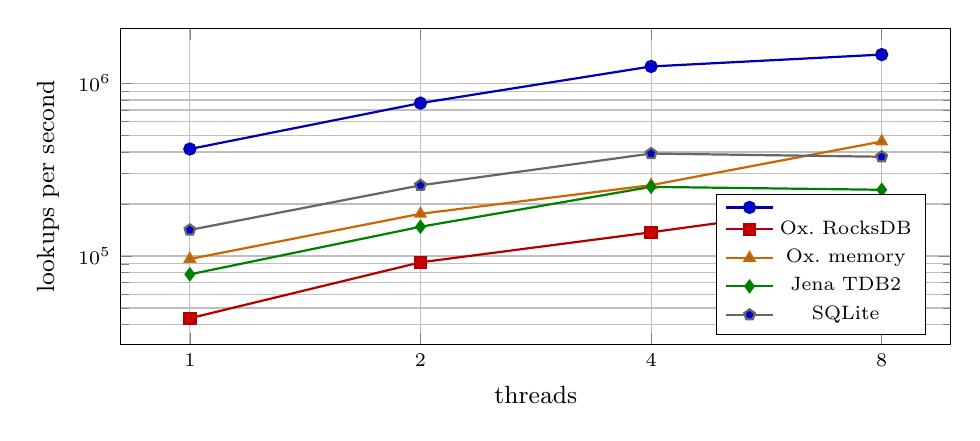
\begin{tikzpicture}
\begin{axis}[width=\columnwidth,height=5.6cm,xmode=log,ymode=log,log basis x=2,xtick={1,2,4,8},xticklabels={1,2,4,8},xlabel={threads},ylabel={lookups per second},grid=both,legend pos=south east,legend style={font=\scriptsize},tick label style={font=\scriptsize},label style={font=\small}]
\addplot+[mark=*,color=blue!70!black,thick] coordinates {(1,416050) (2,767222) (4,1250348) (8,1464779)};
\addlegendentry{\sys{}}
\addplot+[mark=square*,color=red!70!black,thick] coordinates {(1,43594) (2,91866) (4,137110) (8,208977)};
\addlegendentry{Ox.\ RocksDB}
\addplot+[mark=triangle*,color=orange!80!black,thick] coordinates {(1,96048) (2,175432) (4,256917) (8,459776)};
\addlegendentry{Ox.\ memory}
\addplot+[mark=diamond*,color=green!50!black,thick] coordinates {(1,78280) (2,147564) (4,251154) (8,241599)};
\addlegendentry{Jena TDB2}
\addplot+[mark=pentagon*,color=black!60,thick] coordinates {(1,141488) (2,256339) (4,391720) (8,375194)};
\addlegendentry{SQLite}
\end{axis}
\end{tikzpicture}

\caption{Lookups per second on LUBM(10) against the number of threads (both axes logarithmic).}
\label{fig-conc}
\end{figure}

\begin{table}[t]
\caption{Concurrency on LUBM(10): lookups per second with 1 and 8 reader threads, readers' lookups per second with one writer running, and inserts per second with 1 and 8 writer threads (one triple per transaction; \sys's inserts are not logged, and Jena's commit forces the journal to disk). The machine has 8 performance cores.}
\label{tab-conc}
\small
\resizebox{\columnwidth}{!}{%
\begin{tabular}{@{}lrrrrrr@{}}
\toprule
 & \multicolumn{2}{c}{lookups/s} & \multicolumn{2}{c}{readers + 1 writer} & \multicolumn{2}{c}{inserts/s} \\
\cmidrule(lr){2-3}\cmidrule(lr){4-5}\cmidrule(lr){6-7}
Engine & 1 & 8 & 1 & 8 & 1 & 8 \\
\midrule
\sys{} & 416k & 1.46M & 398k & 1.39M & 264k & 950k \\
Ox.\ RocksDB & 44k & 209k & 38k & 136k & 91k & 105k \\
Ox.\ memory & 96k & 460k & 69k & 288k & 679k & 186k \\
Jena TDB2 & 78k & 242k & 22k & 74k & 16 & 15 \\
SQLite & 141k & 375k & 111k & 322k & 15k & 14k \\
\bottomrule
\end{tabular}}
\end{table}


\stitle{Readers}.
\sys serves 416 thousand lookups per second with one thread and 1.46 million
with eight, 3.5 times more, and its single thread already beats every other
engine at eight threads except Oxigraph's in-memory store, which reaches 460
thousand.
At eight threads \sys serves 7.0, 3.2, 6.1, and 3.9 times the lookups of
Oxigraph on RocksDB, Oxigraph in memory, Jena TDB2, and SQLite.
Every engine scales with threads here; \sys's lead is its per-lookup cost, 2.4
microseconds, kept as threads are added.

\stitle{Readers beside a writer}.
With a writer inserting continuously, \sys's eight readers still serve 1.39
million lookups per second, 3.5 times its one-reader rate, while the writer
keeps inserting 111 thousand triples per second.
Beside a writer, eight readers reach 74 thousand lookups per second on Jena
TDB2, 136 thousand on Oxigraph on RocksDB, 288 thousand on Oxigraph in memory,
and 322 thousand on SQLite, so \sys's eight readers do 18.8, 10.2, 4.8, and 4.3
times as many.

\stitle{Writers}.
\sys's insert rate grows from 264 thousand per second with one thread to 950
thousand with eight, 3.6 times; Oxigraph on RocksDB gains 16\%, Oxigraph in
memory loses nearly three quarters, SQLite loses 4\%, and Jena TDB2's rate is bounded by
its commit.
The comparison favors \sys in one respect: its inserts here go through the
store without the write-ahead log, while the other engines commit each insert
with their default durability.
The scaling of \sys's own curve is the result; Oxigraph's in-memory store, which
is not durable either, inserts faster with one thread (679 thousand per
second).

\stitle{What limits it}.
Heavy queries scale less: the 16,000-row $(\cdot,p,o)$ query goes from 148 to 330
queries per second with eight threads, because it copies leaf after leaf and
decodes thousands of terms, so it is bound by memory traffic.
Splits and merges take the pessimistic path and serialize with each other on
the pages they share, and inserts into one leaf serialize on its latch.

\subsection{RQ6: Design Choices}

\stitle{Permutations}.
One tree, SPO, answers a pattern that does not bind the subject by a scan of
the whole tree.
Table~\ref{tab-permstudy} counts, on LUBM(1) with a cold 64-frame pool, the
page reads of a pattern for one, three, and all six permutations (averages
over 20 sampled patterns per shape).
Three permutations cut the pages of $(\cdot,p,\cdot)$ by 7.9$\times$ and those
of $(\cdot,\cdot,o)$ and $(\cdot,p,o)$ by 40$\times$; the other three trees
cost 66\% more space and change no pattern, because every shape already has
a prefix scan in the first three.

\begin{table}[t]
\caption{Page reads per pattern on LUBM(1) (cold 64-frame pool, bulk-loaded) and file size, by set of permutations.}
\label{tab-permstudy}
\small
\begin{tabular}{@{}lrrrr@{}}
\toprule
Permutations & $(\cdot,p,\cdot)$ & $(\cdot,\cdot,o)$ & $(\cdot,p,o)$ & file (MiB) \\
\midrule
SPO & 599 & 599 & 599 & 6.1 \\
SPO, POS, OSP & 76 & 15 & 15 & 10.8 \\
all six & 76 & 15 & 15 & 17.9 \\
\bottomrule
\end{tabular}
\end{table}

\stitle{Bulk loading}.
Loading the 15 files of LUBM(1) one triple at a time takes 1.74\,s and 16.2\,MiB
for three permutations; the bulk loader takes 1.08\,s and 10.8\,MiB, a third
less space, and a full scan reads 599 pages instead of 1,131 because
inserted leaves are about half full and bulk-loaded leaves are full.
With the loader, the time that remains is the dictionary's.

\stitle{Decode cache}.
Table~\ref{tab-cache} shows what the dictionary's decode cache buys:
the subject-bound pattern gets 4.3$\times$ faster, patterns that return
thousands of rows get 1.5 to 2.3$\times$ faster, and the largest instance
queries 2.0$\times$.
The cache does nothing for ids, which is why the
interval scan alone is 6$\times$ faster than the same query returning
strings.
A cache is the remedy Jena uses for the same cost; a cheaper id-to-spelling
access path would help every cold query and is future work.

\begin{table}[t]
\caption{The effect of \sys's decode cache (65\,536 entries) on the time to return strings: mean time per query on LUBM(10), and the instances of a class on the Gene Ontology (30 classes per row).}
\label{tab-cache}
\small
\begin{tabular}{@{}lrrr@{}}
\toprule
Workload & answers & cache off & cache on \\
\midrule
$(s,\cdot,\cdot)$ & 7 & 13\,$\mu$s & 3\,$\mu$s \\
$(s,p,\cdot)$ & 2 & 3\,$\mu$s & 2\,$\mu$s \\
$(\cdot,\cdot,o)$ & 16,233 & 24.9\,ms & 11.0\,ms \\
$(\cdot,p,o)$ & 16,225 & 14.9\,ms & 10.2\,ms \\
$(\cdot,p,\cdot)$ & 70,720 & 113.1\,ms & 70.8\,ms \\
\midrule
instances, 100-999 below & 2,954 & 2.4\,ms & 258\,$\mu$s \\
instances, 1000+ below & 29,904 & 22.6\,ms & 11.5\,ms \\
\bottomrule
\end{tabular}
\end{table}

